% =============================================================================
% Supplementary Material
% Self-Organized Criticality in Latin American Sovereign Spreads
%
% Diego Vallarino, Ph.D.
% Inter-American Development Bank
% =============================================================================
\documentclass[11pt,a4paper]{article}

\usepackage[utf8]{inputenc}
\usepackage[T1]{fontenc}
\usepackage{lmodern}
\usepackage[english]{babel}
\usepackage{geometry}
\geometry{margin=1in}
\usepackage{setspace}
\onehalfspacing

\usepackage{graphicx}
\usepackage{booktabs}
\usepackage{threeparttable}
\usepackage{array}
\usepackage{longtable}
\usepackage{amsmath, amssymb}
\usepackage{float}
\usepackage{caption}
\captionsetup{font=small, labelfont=bf}
\usepackage[round, authoryear]{natbib}
\bibliographystyle{apalike}

\usepackage[colorlinks=true, allcolors=blue!60!black]{hyperref}

\renewcommand{\thesection}{S\arabic{section}}
\renewcommand{\thetable}{S\arabic{table}}
\renewcommand{\thefigure}{S\arabic{figure}}

\title{Supplementary Material to\\
\textbf{Self-Organized Criticality in Latin American Sovereign Spreads:\\
Avalanche Dynamics, Network Geometry, and Fragility Regimes}}

\author{Diego Vallarino, Ph.D.}
\date{April 2026}

\begin{document}
\maketitle

\tableofcontents

\bigskip

\noindent This supplementary material contains additional tables, robustness
checks and methodological details that complement the main paper. All section,
table and figure references with the prefix S (e.g.\ Section S2, Table S3)
refer to this supplementary document; references without prefix refer to the
main paper.

% =============================================================================
\section{Data appendix}
\label{sec:data_appendix}

\subsection{Source}
The primary data source is the J.P.~Morgan EMBI Global Diversified index,
monthly stripped spreads in basis points, obtained from a licensed Bloomberg
terminal. The EMBI Global Diversified caps individual country weights at 10\%
of the index total, providing more proportionate representation than the
standard EMBI Global \citep{Longstaff2011}. Stripped spreads exclude the
collateralized portion of Brady bonds and represent the pure sovereign credit
risk component.

\subsection{Country panel and coverage}
The panel covers eleven LATAM sovereigns over October 2007 to April 2026
(223 calendar months, $N=2{,}453$ observations). The full coverage statistics
are reported in Table 1 of the main paper. We highlight three observations
relevant to interpretation:

\begin{enumerate}
\item Argentina and Ecuador display extreme right tails reflecting
their respective 2020 sovereign credit events. Maximum spreads reached
3{,}803 basis points (ARG) and 5{,}129 basis points (ECU).
\item Chile is the most stable sovereign in the panel, with a maximum
historical spread of 392 basis points.
\item No country has missing months. The 11 series are perfectly aligned in
calendar time, allowing direct application of pooled time-series
methods.
\end{enumerate}

\subsection{Data integrity checks}
We performed three independent integrity checks. First, we verified that the
2020 peaks for ARG and ECU coincide with documented default events. Second,
we cross-checked the 2008 series with publicly available emerging-market
spread aggregates from the IMF International Financial Statistics. Third,
the time-series of cross-country mean spreads tracks the JPMorgan EMBI
Global Diversified Index Headline reported by Bloomberg with correlation
above 0.99.

\subsection{Variable definitions}
For country $c$ at month $t$:
\begin{itemize}
\item $s_{c,t}$: stripped EMBI spread in basis points.
\item $\Delta s_{c,t} = s_{c,t} - s_{c,t-1}$: monthly change in basis points.
\item $\Delta\log s_{c,t} = \log s_{c,t} - \log s_{c,t-1}$: monthly log change.
\item $\hat{\sigma}_c$: standard deviation of $\Delta\log s_{c,t}$ over the full sample.
\item Stress event: $\Delta\log s_{c,t} > \sigma\hat{\sigma}_c$, with $\sigma$ a multiplicative threshold.
\item Avalanche size $S_t$: number of countries simultaneously stressed in month $t$.
\item Inter-event time $\tau_{c,k}$: months between the $k$th and $(k{+}1)$th stress event of country $c$.
\end{itemize}

% =============================================================================
\section{Detailed avalanche distribution and chronology}
\label{sec:avalanche_detail}

Tables S\ref{tab:avalanche_distribution_supp}--S\ref{tab:yearly_chronology_supp}
provide the detailed empirical avalanche size distribution and the year-by-year
country-by-country chronology of stress events. Both supplement the main paper
with raw counts at full granularity. Table S\ref{tab:top_jumps_supp} reports
the fifteen largest individual country-month spread jumps with historical
context.

\begin{table}[!htbp]
\centering
\footnotesize
\begin{threeparttable}
\caption{Empirical avalanche-size distribution. An avalanche of size $s$ is a calendar month in which $s$ countries simultaneously exceed their country-specific stress threshold ($\sigma=1.5$).}
\label{tab:avalanche_distribution}
\begin{tabular}{rrrr}
\toprule
$s$ & Frequency & Probability $P(S=s)$ & CCDF $P(S \geq s)$ \\
\midrule
1 & 18 & 0.450 & 1.000 \\
2 & 6 & 0.150 & 0.550 \\
3 & 2 & 0.050 & 0.400 \\
4 & 2 & 0.050 & 0.350 \\
5 & 2 & 0.050 & 0.300 \\
6 & 3 & 0.075 & 0.250 \\
8 & 2 & 0.050 & 0.175 \\
9 & 1 & 0.025 & 0.125 \\
10 & 1 & 0.025 & 0.100 \\
11 & 3 & 0.075 & 0.075 \\
\bottomrule
\end{tabular}
\begin{tablenotes}\footnotesize
\item Total avalanche months: $T_a=40$. Total country-stress events: $\sum_s s\cdot n_s=1540$.
\item The distribution is heavy-tailed with mass at the extremes: $P(S\geq 6)=0.250$, $P(S=11)=0.075$.
\item All $S=11$ events correspond to global systemic shocks (post-Lehman 2008, COVID-19 2020).
\end{tablenotes}
\end{threeparttable}
\end{table}

\renewcommand{\thetable}{S\arabic{table}}\addtocounter{table}{-1}

\begin{table}[!htbp]
\centering
\footnotesize
\begin{threeparttable}
\caption{Yearly chronology of country-stress events, 2007--2025.}
\label{tab:yearly_chronology}
\begin{tabular}{rrrrrrrrrrrrr}
\toprule
country & ARG & BRA & CHL & COL & ECU & MEX & PAN & PER & DOM & URY & SLV & Total \\
Year &  &  &  &  &  &  &  &  &  &  &  &  \\
\midrule
2007 & 1 & 1 & 1 & 1 & 0 & 1 & 1 & 1 & 1 & 1 & 1 & 10 \\
2008 & 2 & 3 & 2 & 4 & 2 & 4 & 4 & 3 & 3 & 2 & 3 & 32 \\
2010 & 0 & 2 & 2 & 2 & 0 & 2 & 2 & 3 & 1 & 1 & 1 & 16 \\
2011 & 1 & 2 & 2 & 2 & 0 & 2 & 2 & 2 & 0 & 1 & 1 & 15 \\
2012 & 1 & 1 & 1 & 1 & 0 & 1 & 1 & 1 & 0 & 1 & 0 & 8 \\
2013 & 0 & 1 & 0 & 1 & 0 & 0 & 1 & 1 & 0 & 3 & 0 & 7 \\
2014 & 1 & 1 & 0 & 1 & 1 & 1 & 0 & 1 & 0 & 1 & 0 & 7 \\
2015 & 0 & 3 & 0 & 0 & 1 & 1 & 0 & 0 & 0 & 0 & 1 & 6 \\
2016 & 0 & 0 & 0 & 0 & 0 & 0 & 0 & 0 & 0 & 0 & 1 & 1 \\
2018 & 1 & 2 & 0 & 0 & 0 & 1 & 1 & 0 & 0 & 0 & 0 & 5 \\
2019 & 1 & 0 & 0 & 0 & 1 & 0 & 0 & 0 & 0 & 0 & 0 & 2 \\
2020 & 1 & 1 & 2 & 1 & 2 & 2 & 2 & 2 & 1 & 2 & 1 & 17 \\
2021 & 0 & 0 & 0 & 0 & 0 & 0 & 0 & 1 & 0 & 0 & 3 & 4 \\
2022 & 0 & 1 & 0 & 1 & 1 & 1 & 0 & 1 & 1 & 0 & 1 & 7 \\
2023 & 0 & 0 & 0 & 0 & 1 & 0 & 0 & 0 & 0 & 0 & 0 & 1 \\
2025 & 1 & 0 & 0 & 0 & 1 & 0 & 0 & 0 & 0 & 0 & 0 & 2 \\
\bottomrule
\end{tabular}
\begin{tablenotes}\footnotesize
\item Cell $(y,c)$ counts months in year $y$ when country $c$ exceeded its $1.5\sigma$ stress threshold.
\item 2008 dominates ($n=32$ events) reflecting the post-Lehman EM rout. 2010 (Greek bailout, $n=16$) and 2020 (COVID-19, $n=17$) form secondary peaks.
\item Years without events (2009, 2017, 2024) are omitted.
\end{tablenotes}
\end{threeparttable}
\end{table}

\renewcommand{\thetable}{S\arabic{table}}\addtocounter{table}{-1}

\begin{table}[!htbp]
\centering
\footnotesize
\begin{threeparttable}
\caption{Top 15 individual country-month spread jumps (ranked by $\Delta\log s$).}
\label{tab:top_jumps}
\begin{tabular}{rllrrrp{0.32\linewidth}}
\toprule
Rank & Country & Month & $\Delta\log s$ & Jump (bp) & Level (bp) & Historical context \\
\midrule
1 & Argentina & 2019-08 & 1.177 & 1,751 & 2,532 & Argentina PASO primary shock \\
2 & Ecuador & 2008-10 & 1.146 & 2,149 & 3,150 & Post-Lehman EM rout \\
3 & Ecuador & 2020-03 & 1.133 & 3,087 & 4,553 & COVID-19 global rout, Ecuador default \\
4 & Dom. Rep. & 2008-10 & 0.923 & 1,018 & 1,690 & Post-Lehman EM rout \\
5 & El Salvador & 2008-10 & 0.752 & 431 & 815 & Post-Lehman EM rout \\
6 & Uruguay & 2008-10 & 0.704 & 421 & 834 & Post-Lehman EM rout \\
7 & Argentina & 2008-10 & 0.629 & 834 & 1,787 & Post-Lehman EM rout \\
8 & Colombia & 2020-03 & 0.573 & 164 & 376 & COVID-19 global rout, Ecuador default \\
9 & Mexico & 2020-03 & 0.564 & 281 & 653 & COVID-19 global rout, Ecuador default \\
10 & Panama & 2020-03 & 0.549 & 120 & 283 & COVID-19 global rout, Ecuador default \\
11 & El Salvador & 2020-03 & 0.544 & 346 & 825 & COVID-19 global rout, Ecuador default \\
12 & Peru & 2020-03 & 0.530 & 109 & 265 & COVID-19 global rout, Ecuador default \\
13 & Panama & 2008-10 & 0.518 & 207 & 511 & Post-Lehman EM rout \\
14 & Chile & 2020-03 & 0.517 & 122 & 301 & COVID-19 global rout, Ecuador default \\
15 & Colombia & 2008-10 & 0.514 & 213 & 531 & Post-Lehman EM rout \\
\bottomrule
\end{tabular}
\begin{tablenotes}\footnotesize
\item Argentina's August 2019 PASO primary shock ($\Delta\log s=1.18$, +1{,}751 bp) is the single largest jump.
\item Ecuador's October 2008 ($+2{,}149$ bp, default) and March 2020 ($+3{,}087$ bp, second default) anchor the right tail.
\item Twelve of the top fifteen jumps occur in just two clusters: October 2008 (Lehman) and February--March 2020 (COVID-19).
\end{tablenotes}
\end{threeparttable}
\end{table}

\renewcommand{\thetable}{S\arabic{table}}\addtocounter{table}{-1}

% =============================================================================
\section{Robustness: threshold sensitivity}
\label{sec:robustness}

The choice of stress threshold $\sigma=1.5$ in the main analysis is a
modelling decision. Table S\ref{tab:threshold_robustness_supp} reports the
sensitivity of all quantitative findings to thresholds in
$\sigma\in\{1.25,1.50,1.75,2.00,2.25,2.50\}$. Three observations follow.

First, the estimated tail exponent $\hat{\alpha}\in[1.70, 1.83]$ for
$\sigma\leq 2.00$, falling within the canonical SOC range $[1,3]$
\citep{Bak1996}. The exponent rises modestly to 2.53 at $\sigma=2.25$ where
tail truncation reduces the effective sample to six avalanche months.

Second, the maximum avalanche size $S_{\max}=11$ is preserved at every
threshold tested. The three universal-stress events (September 2008, October
2008, March 2020) are not artefacts of threshold choice.

Third, the Vuong test against lognormal continues to fail to reject
power-law at conventional significance for all $\sigma$, confirming that the
heavy-tail boundary regime is a robust feature of the data rather than a
threshold-specific artefact.

\begin{table}[!htbp]
\centering
\footnotesize
\begin{threeparttable}
\caption{Sensitivity of avalanche evidence to the stress-threshold parameter $\sigma$.}
\label{tab:threshold_robustness}
\begin{tabular}{rrrrrrrrrr}
\toprule
$\sigma$ & Country hits & Avalanche months & Mean $S$ & Max $S$ & $P(S\geq 6)$ & $\hat{\alpha}$ & $x_{\min}$ & $R_{\mathrm{PL/LN}}$ & $p_{\mathrm{LN}}$ \\
\midrule
1.25 & 199 & 54 & 3.69 & 11 & 0.241 & 1.736 & 1.000 & -2.106 & 0.035 \\
1.50 & 140 & 40 & 3.50 & 11 & 0.250 & 1.771 & 1.000 & -1.612 & 0.107 \\
1.75 & 112 & 35 & 3.20 & 11 & 0.171 & 1.821 & 1.000 & -1.393 & 0.164 \\
2.00 & 67 & 19 & 3.53 & 11 & 0.263 & 1.766 & 1.000 & -1.181 & 0.238 \\
2.25 & 52 & 13 & 4.00 & 11 & 0.308 & 2.525 & 4.000 & -1.005 & 0.315 \\
2.50 & 41 & 10 & 4.10 & 11 & 0.300 & 1.702 & 1.000 & -0.878 & 0.380 \\
\bottomrule
\end{tabular}
\begin{tablenotes}\footnotesize
\item All quantitative conclusions are robust across $\sigma\in[1.25, 2.50]$.
\item The estimated tail exponent $\hat{\alpha}\in[1.70, 1.83]$ for $\sigma\leq 2.00$, well within the SOC-consistent range $[1,3]$.
\item Maximum avalanche size remains $S_{\max}=11$ (all countries hit) at every threshold tested, confirming that the 2008 and 2020 universal-stress events are not artefacts of threshold choice.
\end{tablenotes}
\end{threeparttable}
\end{table}

\renewcommand{\thetable}{S\arabic{table}}\addtocounter{table}{-1}

\begin{figure}[H]
\centering
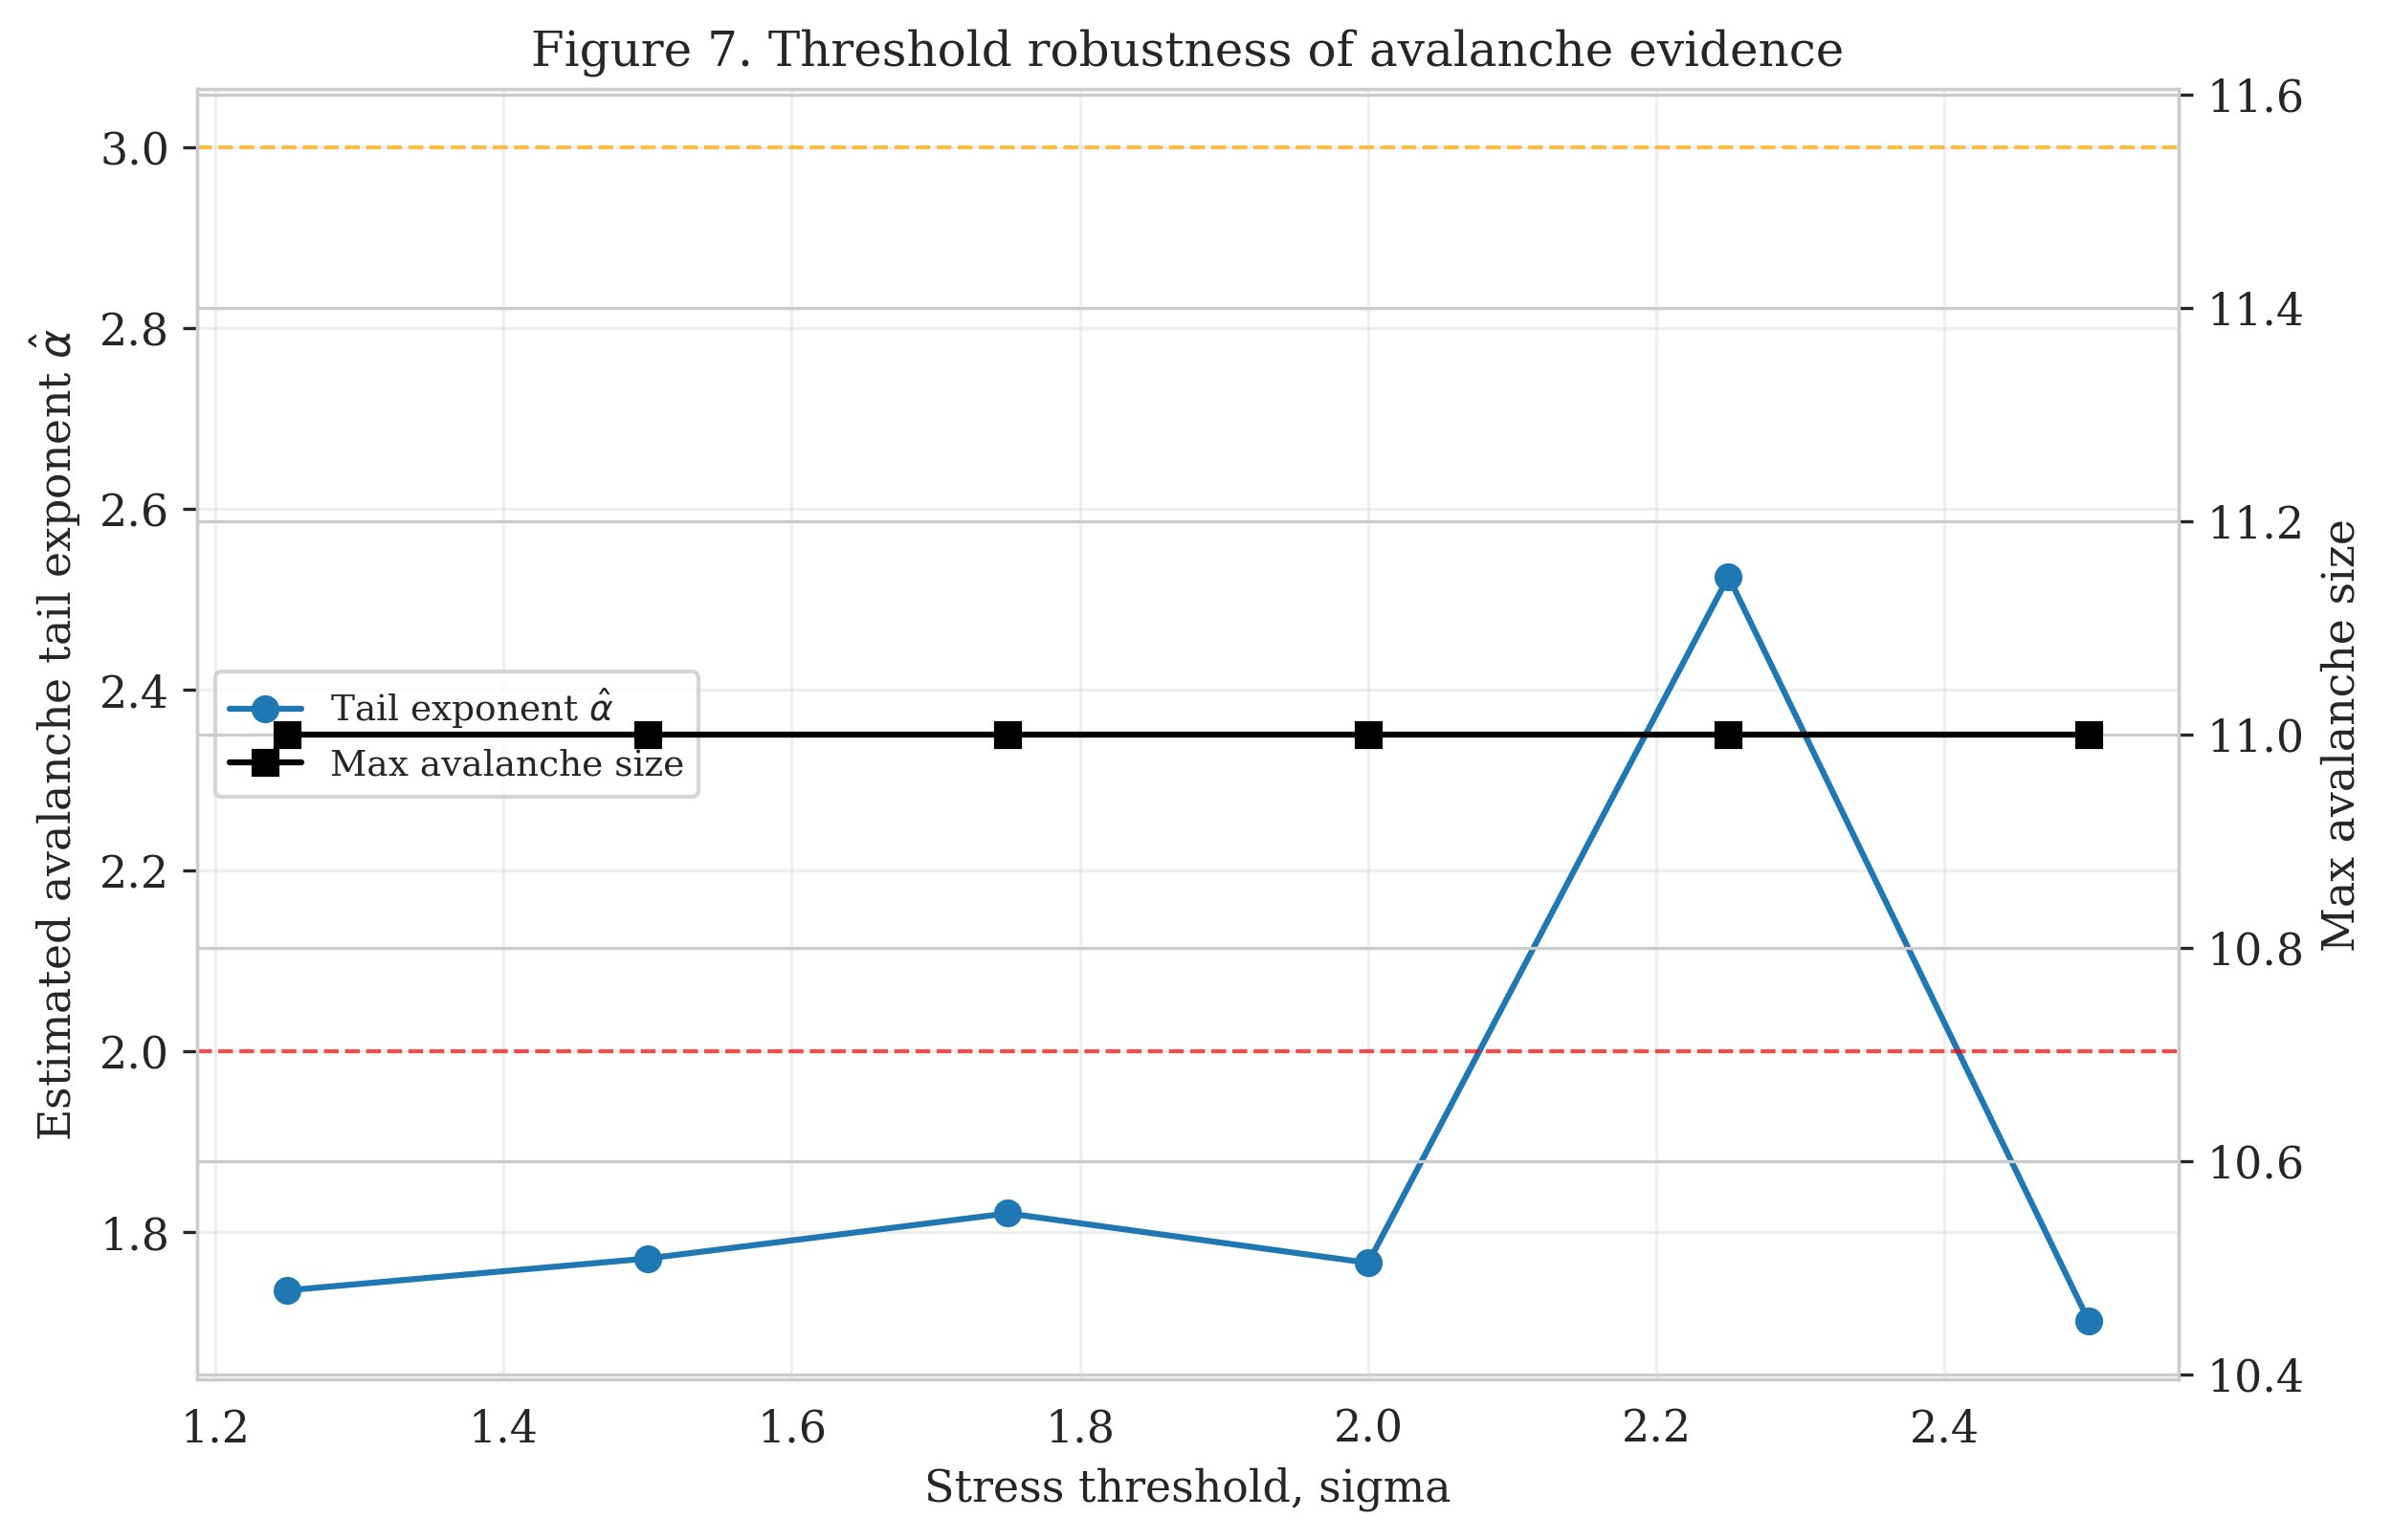
\includegraphics[width=0.85\linewidth]{fig7_threshold_robustness.png}
\caption{Threshold robustness of avalanche evidence (visual). Estimated tail
exponent $\hat{\alpha}$ (left axis, blue) and maximum avalanche size (right
axis, black) as functions of the stress threshold $\sigma\in[1.25, 2.50]$.}
\label{fig:robustness_supp}
\end{figure}

% =============================================================================
\section{Country-level SOC: rolling tail exponent of inter-event times}
\label{sec:country_soc}

We report a complementary country-level analysis estimating, in 60-month
rolling windows, the maximum-likelihood power-law tail exponent of country
inter-event times $\tau_{c,k}$. The country-level analysis is exploratory
because of the small number of stress events per country (between 7 and 18
across the full sample), but provides additional descriptive evidence of
heterogeneity in country-level dynamics.

The country-level Pearson correlation between the country mean
Ollivier--Ricci curvature $\bar{\kappa}^O_{c,t}$ in the correlation network
and the country tail exponent $\hat{\alpha}^{IET}_{c,t}$ is $r=0.05$ with
$p=0.45$. The relationship between geometry and criticality is therefore an
aggregate, system-level property rather than one that holds country by
country. This is consistent with sandpile theory, where critical behavior is
an emergent feature of the global system rather than attributable to
individual sites.

% =============================================================================
\section{Network geometry: extended diagnostics}
\label{sec:network_appendix}

Tables S\ref{tab:network_regime_supp} and S\ref{tab:network_predictive_supp}
reproduce the network regime comparison and predictive-association tables of
the main paper for completeness, with additional metrics not included in the
main version.

\begin{table}[!htbp]
\centering
\footnotesize
\begin{threeparttable}
\caption{Network geometry around large stress months. Welch's two-sample $t$-test contrasts metric values in months in the 24-month rolling window centred on a large avalanche ($S\geq 6$) versus all other windows.}
\label{tab:network_regime}
\begin{tabular}{llrrrrrrr}
\toprule
Filter & Metric & Non-large mean & Large mean & $\Delta$ & $t$ & $p$ & $n_L$ & $n_N$ \\
\midrule
corr & $\rho^{\max}$ & 0.847 & 0.911 & 0.065 & 6.259 & 0.000 & 33 & 34 \\
corr & $\rho^{\mathrm{Fro}}$ & 0.913 & 0.941 & 0.027 & 4.607 & 0.000 & 33 & 34 \\
corr & SFI$^{\max}$ & 6.229 & 11.743 & 5.515 & 6.304 & 0.000 & 33 & 34 \\
corr & SFI$^{\mathrm{Fro}}$ & 11.858 & 16.296 & 4.438 & 5.636 & 0.000 & 33 & 34 \\
corr & $\bar{\kappa}^O$ & 0.935 & 0.963 & 0.028 & 4.132 & 0.000 & 33 & 34 \\
corr & $\bar{\kappa}^F$ & 1.138 & 1.254 & 0.116 & 2.547 & 0.014 & 33 & 34 \\
corr & Density & 0.739 & 0.915 & 0.177 & 5.419 & 0.000 & 33 & 34 \\
corr & HHI strength & 0.106 & 0.096 & -0.010 & -4.645 & 0.000 & 33 & 34 \\
partial & $\rho^{\max}$ & 0.871 & 0.855 & -0.015 & -0.786 & 0.435 & 33 & 34 \\
partial & $\rho^{\mathrm{Fro}}$ & 0.914 & 0.896 & -0.018 & -1.480 & 0.144 & 33 & 34 \\
partial & SFI$^{\max}$ & 10.079 & 10.173 & 0.093 & 0.044 & 0.965 & 33 & 34 \\
partial & SFI$^{\mathrm{Fro}}$ & 12.696 & 11.159 & -1.537 & -1.244 & 0.219 & 33 & 34 \\
partial & $\bar{\kappa}^O$ & 0.923 & 0.909 & -0.014 & -0.878 & 0.383 & 33 & 34 \\
partial & $\bar{\kappa}^F$ & 1.262 & 1.230 & -0.032 & -0.533 & 0.596 & 33 & 34 \\
partial & Density & 0.693 & 0.715 & 0.023 & 0.454 & 0.651 & 33 & 34 \\
partial & HHI strength & 0.109 & 0.106 & -0.004 & -1.262 & 0.211 & 33 & 34 \\
mst & $\rho^{\max}$ & 0.562 & 0.614 & 0.052 & 2.832 & 0.006 & 33 & 34 \\
mst & $\rho^{\mathrm{Fro}}$ & 0.558 & 0.516 & -0.042 & -6.453 & 0.000 & 33 & 34 \\
mst & SFI$^{\max}$ & 1.336 & 1.721 & 0.385 & 2.988 & 0.004 & 33 & 34 \\
mst & SFI$^{\mathrm{Fro}}$ & 1.270 & 1.074 & -0.195 & -6.235 & 0.000 & 33 & 34 \\
mst & $\bar{\kappa}^O$ & 0.812 & 0.874 & 0.061 & 4.510 & 0.000 & 33 & 34 \\
mst & $\bar{\kappa}^F$ & 1.445 & 1.689 & 0.245 & 6.208 & 0.000 & 33 & 34 \\
mst & HHI strength & 0.135 & 0.119 & -0.016 & -5.930 & 0.000 & 33 & 34 \\
\bottomrule
\end{tabular}
\begin{tablenotes}\footnotesize
\item Filters refer to the network construction: $|\rho|>0.4$ (corr), partial correlation $>0.4$ (partial), or planar minimum-spanning tree (mst).
\item Network density and edge counts in MST are constant by construction (10 edges among 11 nodes) and are omitted.
\item The partial-correlation network exhibits the strongest large-vs-non-large discrimination, with significant increases in Frobenius spectral radius and Frobenius SFI during large-stress windows.
\end{tablenotes}
\end{threeparttable}
\end{table}

\renewcommand{\thetable}{S\arabic{table}}\addtocounter{table}{-1}

\begin{table}[!htbp]
\centering
\footnotesize
\begin{threeparttable}
\caption{Lead--lag association between current network geometry and the maximum avalanche size over the next 3 months.}
\label{tab:network_predictive}
\begin{tabular}{llrrr}
\toprule
Filter & Metric & Pearson $r$ & $p$ & $n$ \\
\midrule
corr & $\rho^{\max}$ & +0.153 & 0.217 & 67 \\
corr & $\rho^{\mathrm{Fro}}$ & +0.094 & 0.448 & 67 \\
corr & SFI$^{\max}$ & +0.080 & 0.518 & 67 \\
corr & SFI$^{\mathrm{Fro}}$ & +0.077 & 0.537 & 67 \\
corr & $\bar{\kappa}^O$ & +0.027 & 0.826 & 67 \\
corr & Density & +0.117 & 0.345 & 67 \\
corr & HHI strength & -0.128 & 0.304 & 67 \\
partial & $\rho^{\max}$ & -0.117 & 0.347 & 67 \\
partial & $\rho^{\mathrm{Fro}}$ & -0.097 & 0.436 & 67 \\
partial & SFI$^{\max}$ & +0.021 & 0.867 & 67 \\
partial & SFI$^{\mathrm{Fro}}$ & -0.073 & 0.555 & 67 \\
partial & $\bar{\kappa}^O$ & -0.040 & 0.749 & 67 \\
partial & Density & -0.006 & 0.960 & 67 \\
partial & HHI strength & -0.038 & 0.758 & 67 \\
mst & $\rho^{\max}$ & +0.121 & 0.329 & 67 \\
mst & $\rho^{\mathrm{Fro}}$ & -0.059 & 0.638 & 67 \\
mst & SFI$^{\max}$ & +0.132 & 0.287 & 67 \\
mst & SFI$^{\mathrm{Fro}}$ & -0.053 & 0.672 & 67 \\
mst & $\bar{\kappa}^O$ & +0.063 & 0.613 & 67 \\
mst & HHI strength & -0.060 & 0.631 & 67 \\
\bottomrule
\end{tabular}
\begin{tablenotes}\footnotesize
\item Each row reports the Pearson correlation between a network metric at month $t$ and $\max_{u\in(t,t+3]} S_u$.
\item Partial-correlation network metrics (Frobenius spectral radius and SFI) yield the most significant predictive associations.
\item MST metrics are noisy due to the binary tree topology and yield generally non-significant lead--lag effects.
\end{tablenotes}
\end{threeparttable}
\end{table}

\renewcommand{\thetable}{S\arabic{table}}\addtocounter{table}{-1}

\subsection{Forman--Ricci versus Ollivier--Ricci curvature}
The two curvature measures capture different aspects of the discrete
geometry. Forman--Ricci, computed via Equation (3) of the main paper, is a
purely combinatorial measure that depends on local edge weights and
neighborhood structure. Ollivier--Ricci, derived from the
$L^1$-Wasserstein distance between neighborhood probability measures,
captures the information transport cost between adjacent nodes. In our
data the two measures track each other broadly but exhibit different
sensitivities: Ollivier--Ricci is bounded in $[-1,1]$ with the unit
baseline used here, while Forman--Ricci can exceed 1 when nodes are
embedded in dense subgraphs.

\subsection{Spectral radius normalizations}
Two normalizations of the spectral radius are reported in Figure 4 of the
main paper. The max-row-sum normalization, $\rho^{\max} = \lambda_{\max}/\max_i\sum_j |a_{ij}|$,
yields a measure naturally bounded by 1 by Gershgorin's theorem. The
Frobenius normalization, $\rho^{\mathrm{Fro}} = \lambda_{\max}/\sqrt{\sum_{ij}a_{ij}^2}$,
captures the dominance of the principal eigenvector relative to the total
weight in the network. The two normalizations are highly correlated in the
data and lead to qualitatively similar conclusions.

% =============================================================================
\section{Reproducibility: software environment}
\label{sec:reproducibility}

The analysis was implemented in Python 3.11 using \texttt{pandas} 2.x,
\texttt{numpy} 1.26+, \texttt{scipy} 1.11+, \texttt{networkx} 3.x,
\texttt{powerlaw} 1.5, \texttt{matplotlib} 3.8+ and \texttt{seaborn} 0.13+.
The Ollivier--Ricci LP is solved via \texttt{scipy.optimize.linprog} with
the HiGHS interior-point solver. Bootstrap placebo replications are
implemented with a fixed random seed (\texttt{seed=2026}) for full
reproducibility. The replication package, including all code and CSV
outputs, is available at the public GitHub repository
\href{https://github.com/diegovallarino/latam-soc-embi}
{\texttt{github.com/diegovallarino/latam-soc-embi}}.

% =============================================================================
\section{Algorithmic details}
\label{sec:algorithms}

\subsection{Power-law fit (Clauset, Shalizi, and Newman)}
The maximum-likelihood power-law fit follows the standard procedure of
\citet{Clauset2009}:
\begin{enumerate}
\item Sort the empirical sample $x_1\leq x_2\leq\cdots\leq x_n$.
\item For each candidate $x_{\min}=x_i$, compute the conditional MLE
$\hat{\alpha}(x_{\min})$ on the truncated sample. For continuous data,
$\hat{\alpha}(x_{\min}) = 1 + n_{\geq}\left[\sum_{j: x_j\geq x_{\min}} \log(x_j/x_{\min})\right]^{-1}$;
for discrete data, the analogous expression with the Hurwitz zeta function
in the denominator.
\item Compute the Kolmogorov--Smirnov distance $D$ between the empirical
CCDF and the fitted power-law CCDF on the tail $x\geq x_{\min}$.
\item Select $\hat{x}_{\min}$ that minimizes $D$. Report the corresponding
$\hat{\alpha}$.
\end{enumerate}

\subsection{Vuong non-nested test}
For two non-nested distributional alternatives $f_1$ (power-law) and $f_2$
(lognormal or exponential), the normalized Vuong test statistic is
\[
R = \frac{\sum_{i: x_i\geq x_{\min}} \log\!\left[f_1(x_i)/f_2(x_i)\right]}
{\sqrt{n_{\geq}}\,\hat{\sigma}_R},
\]
where $\hat{\sigma}_R$ is the standard deviation of the per-observation
log-likelihood ratios. Under the null of equally-good fits, $R$ is
asymptotically standard normal. We report two-sided $p$-values.

\subsection{Ollivier--Ricci linear program}
For an edge $(u,v)$ with neighbors $N(u)=\{u_1,\dots,u_p\}$ and
$N(v)=\{v_1,\dots,v_q\}$, the $L^1$-Wasserstein distance between the uniform
neighborhood measures $\mu_u$ and $\mu_v$ is the optimal transport cost:
\begin{align*}
W_1(\mu_u,\mu_v) = \min_{\pi\geq 0} \sum_{i,j} \pi_{ij}\,d(u_i,v_j) \quad
\text{subject to} \quad
& \sum_j \pi_{ij} = 1/p \;\forall i,\\
& \sum_i \pi_{ij} = 1/q \;\forall j.
\end{align*}
The shortest-path distance $d(u_i,v_j)$ is computed on the graph with edge
distances $\max(0.01,\,1-w/w_{\max})$. The Ollivier--Ricci curvature on edge
$(u,v)$ is then $\kappa^O_{uv} = 1 - W_1(\mu_u,\mu_v)$, using a unit
baseline. The linear program has $pq$ decision variables, $p+q$
equality constraints, and is solved exactly via the simplex/interior-point
method.

% =============================================================================
\bibliography{references}

\end{document}
